% Chapter 4
\chapter{Results and conclusion} % Write in your own chapter title
\label{Chapter4}
\indent In this section we discuss results of different evaluations and
also how does our implementation compares with others. We also draw
conclusions and future works to be done.
\section{Results}
\indent From Fig.~\ref{bg_compare}, we infer that Vibe is
computationally very efficient compared to other.  We target human
detection based on its skeleton motion. We have seen different skeleton
output in Fig.~\ref{skeletons}. We have also seen that star skeleton
provides a simple way for leg motion analysis. Therefore we have used
Vibe~\cite{9} as background subtracter and \textbf{Skel}etonized
\textbf{M}otion \textbf{A}nalysis (SKELMOT) based on star skeleton for
object detection in our final implementation.\\
\indent We conclude that with our implementation, system is able to
detect a moving person after it's 3 steps move.
Fig.~\ref{pipeline_images} shows output images at different stages of
pipeline.\\

\begin{figure}[!b]
\centering
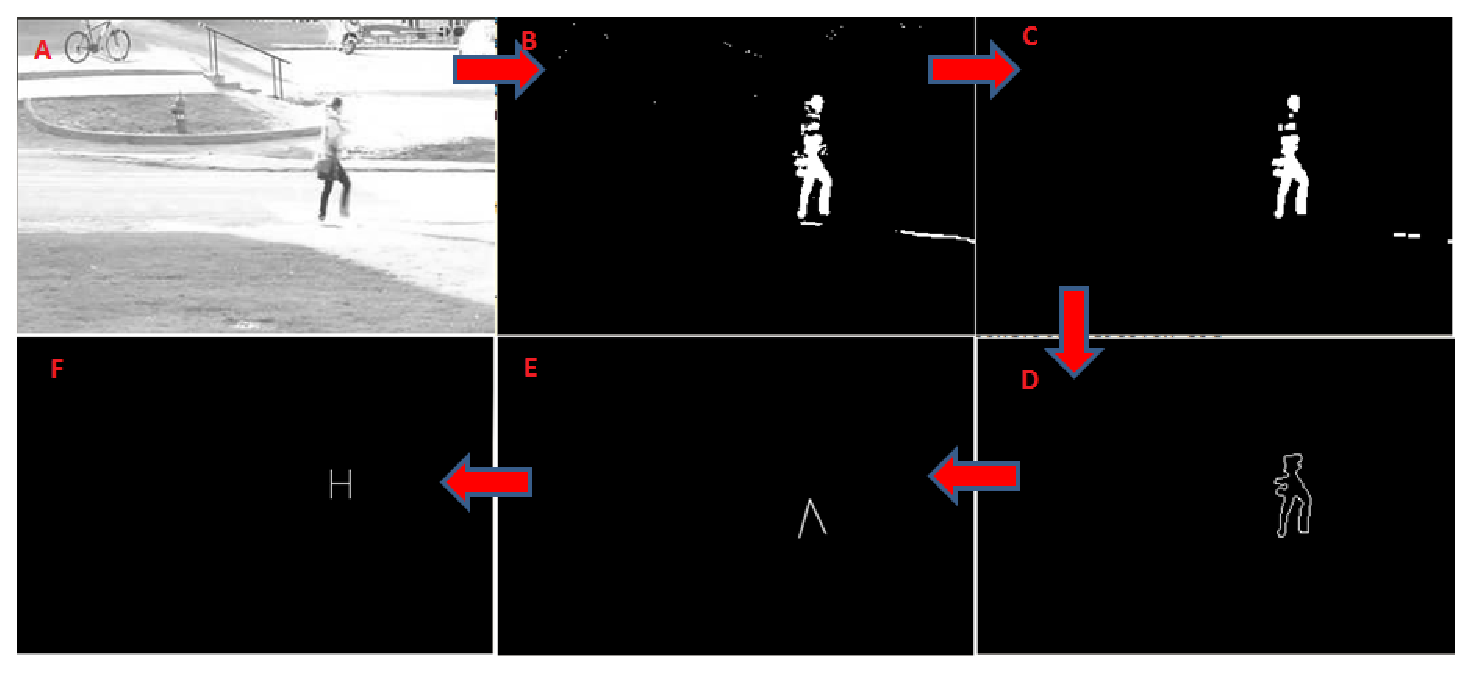
\includegraphics[height=200pt]{Figures/pipeline_images}
\caption{Images at different stages of implementation. (From top left in
clockwise order) \textbf{a.} Gray Scale input frame
\textbf{b.}Foreground extracted image using Vibe \textbf{c.} Cleaned
image \textbf{d.} Contour of moving object \textbf{e.} Plot of 3 points
of interest, centroid and two distance peaks nearer to bottom left and
bottom right corner of bounding box \textbf{f.} Virtual representation
of scene} 
\label{pipeline_images}
\end{figure}
\indent We have also done experiments with negative images like a person
moving on bicycle, or a vehicle moving on road. SKELMOT is successfully able
to discriminate between these objects. Fig.\ref{negative_inputs} shows
how it rejects moving vehicle and bicycle and  does not detect them as
human.\\

\begin{figure}[!b]
\centering
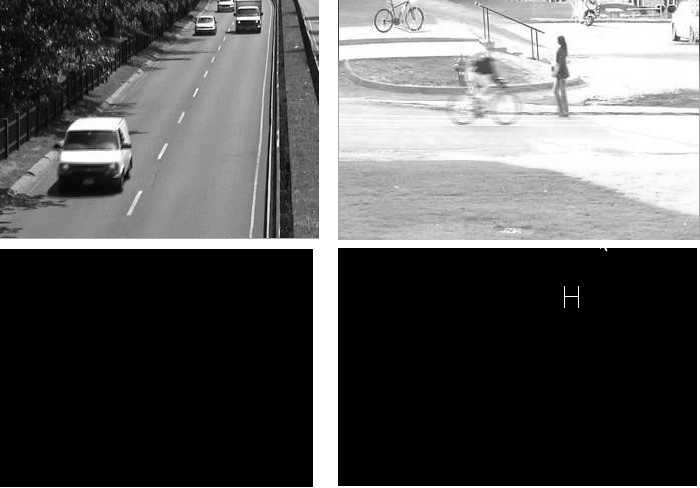
\includegraphics[height=300pt]{Figures/negative_inputs}
\caption{Input and output of pipeline in case of negative images}
\label{negative_inputs}
\end{figure}

\indent We have implemented and executed SKELMOT, Haar-like~\cite{19} and
covariance~\cite{19} feature based detection algorithm on both x86
desktop computer and embedded ARM platform. Comparison of execution time
has been shown in Fig.\ref{pipeline_execution_time}. It shows a
definite improvement in execution speed of SKELMOT over HAAR and covariance
feature based approach.  SKELMOT takes just 3.6 ms on the average, while
HAAR and covariance feature based algorithm take around 20 ms and 248 ms
respectively per frame on x86 platform having DMIPS = 800. Comparison of
timing on ARM platform with DMIPS = 44 shows that SKELMOT takes 182 ms
on the average, while HAAR and covariance feature based algorithm take
around 942 ms and 4.65 s respectively per frame.  \\
\begin{figure}[!h]
\centering
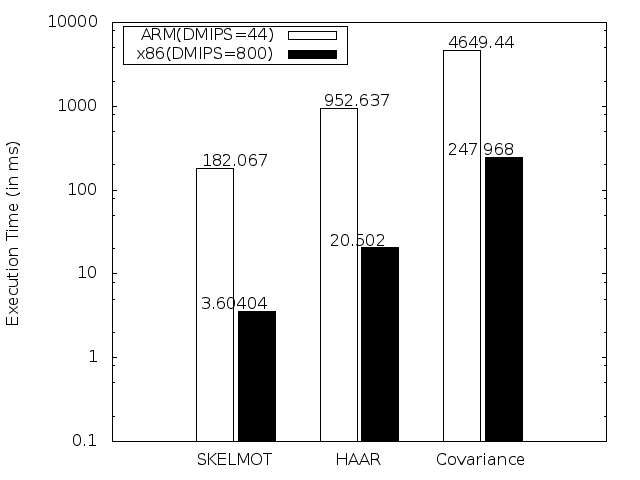
\includegraphics[scale=0.30]{Figures/pipeline_execution_time}
\caption{Execution time of evaluated algorithms on ARM and x86
platform}
\label{pipeline_execution_time}
\end{figure}
\section{Conclusion}
\indent We have seen that method based on covariance or Haar-liek
descriptor is very slow in comparison with skeleton motion descriptor.
Therefore, if a surveillance application requires to identify moving
person, then we might not need to use complex algorithm to get real time
performance with low cost embedded platform. By using proposed
algorithm, we can save a lot of computational power. However, if we wish
to detect human from still frame, then we need to go for other methods.
To use other methods such as haar or covariance features based
descriptor in real time environment, we recommend to implement them in
hardware. This dedicated hardware can further be used with low end
micro-controller to achieve end result.
\section{Future work}
Future work may be carried in following directions:
\begin{enumerate}
\item Test of this algorithm with real camera connected and Zigbee
network will provide good confidence to use it.
\item A research work may be initiated to see actual power saving using
such a low complexity pipeline.
\item There can be improvement in blob tracking algorithm to predict
next position on the basis of past N number of frames.
\item We have seen that low end micro-controller is not able to work with
single frame human detection algorithms. These algorithm can either run on
high performance CPU, or GPU. A work can be initiated to implement such
algorithms in hardware and then to use this hardware with low end
micro-controller. It would be interesting to see difference between power
consumption of two systems.
\item 
\end{enumerate}



